\documentclass{article}

% Required packages
\usepackage{amssymb}
\usepackage{amsmath}
\usepackage{graphicx}
\usepackage{geometry}
\usepackage{tikz}
\usepackage{array}
\usepackage{booktabs}
\usepackage{enumitem}
\usepackage{listings}
\usepackage{xcolor}
\usepackage{fancyhdr}
\usepackage{float}
\usepackage{subcaption}
\usepackage{comment}

\usetikzlibrary{angles, quotes}

% Set page geometry
\geometry{a4paper, margin=1in}

% Configure listings for Python
\lstset{
  language=Python,
  basicstyle=\ttfamily\footnotesize,
  numbers=left,
  numberstyle=\tiny\color{gray},
  frame=single,
  breaklines=true,
  breakatwhitespace=true,
  captionpos=b,
  tabsize=4,
  showspaces=false,
  showstringspaces=false,
  showtabs=false,
  commentstyle=\color{gray}\textit,
  keywordstyle=\color{blue}\bfseries,
  stringstyle=\color{red}
}

\begin{document}

\pagestyle{fancy}
\chead{DSC 257: Unsupervised Learning (Fall 2025)}
\lhead{Homework 2}
\rhead{Randall Rogers}

%------------------
% Solution for 1(a) 
%------------------
\subsection*{Solution 1}
\noindent\rule{\textwidth}{0.4pt}\\

\subsubsection*{Solution 1 (a)}
\subsubsection*{Define $\ell_1$}
\parbox{\textwidth}{
The $\ell_1$ or $||x||_1$ is defined as:
$$\ell_{1} = ||x||_1 = \sum_{i=1}^{d} |x_{i}| $$
}
\subsubsection*{Compute $\ell_1$}
\parbox{\textwidth}{
Let $x=\begin{bmatrix} 1 \\ -2 \\ 3 \end{bmatrix}$ \\

\begin{align*}
  ||x||_1 &= \sum_{i=1}^{3} |x_{i}| \\
  &= |x_{1}| + |x_{2}| + |x_{3}| \\
  &= |1| + |-2| + |3| \\
  &= 1 + 2 + 3 \\
  &= 6
\end{align*}
}


\subsubsection*{\normalfont}{$\therefore$ $||x||_{1} = 6$}

\noindent\rule{\textwidth}{0.4pt}\\

\newpage

%------------------
% Solution for 1(b) 
%------------------
\subsection*{Solution 1}
\noindent\rule{\textwidth}{0.4pt}\\

\subsubsection*{Solution 1 (b)}
\subsubsection*{Define $\ell_2$}
\parbox{\textwidth}{
The $\ell_2$ or $||x||_2$ is defined as:
$$\ell_{2} = ||x||_2 = \sqrt{\sum_{i=1}^{d} x_{i}^2} $$
}
\subsubsection*{Compute $\ell_2$}
\parbox{\textwidth}{
Let $x=\begin{bmatrix} 1 \\ -2 \\ 3 \end{bmatrix}$ \\

\begin{align*}
  ||x||_2 &= \sqrt{\sum_{i=1}^{3} x_{i}^{2}} \\
  &= \sqrt{x_{1}^2 + x_{2}^{2} + x_{3}^{2}} \\
  &= \sqrt{1^{2} + (-2)^{2} + 3^{2}} \\
  &= \sqrt{1 + 4 + 9} \\
  &= \sqrt{14}
\end{align*}
}


\subsubsection*{\normalfont}{$\therefore$ $||x||_{2} = \sqrt{14}$}

\noindent\rule{\textwidth}{0.4pt}\\

\newpage

%------------------
% Solution for 1(c) 
%------------------
\subsection*{Solution 1}
\noindent\rule{\textwidth}{0.4pt}\\

\subsubsection*{Solution 1 (c)}
\subsubsection*{Define $\ell_{\infty}$}
\parbox{\textwidth}{
The $\ell_{\infty}$ or $||x||_{\infty}$ is defined as:
$$\ell_{\infty} = ||x||_{\infty} = \text{max}_{i}\left|x_{i}\right| $$
}
\subsubsection*{Compute $\ell_{\infty}$}
\parbox{\textwidth}{
Let $x=\begin{bmatrix} 1 \\ -2 \\ 3 \end{bmatrix}$ \\

\begin{align*}
  ||x||_{\infty} &= \text{max}(\{|x_{1}|,|x_{2}|,|x_{3}|\}) \\
  &= \text{max}(\{|1|,|-2|,|3|\}) \\
  &= \text{max}(\{1,2,3\}) \\
  &= 3 \\
\end{align*}
}

\subsubsection*{\normalfont}{$\therefore$ $||x||_{\infty} = 3$}

\noindent\rule{\textwidth}{0.4pt}\\

\newpage


%------------------
% Solution for 2(a)
%------------------
\subsection*{Solution 2}
\noindent\rule{\textwidth}{0.4pt}\\
\subsubsection*{Solution 2 (a)}

\subsubsection*{Define $\ell_{2}$ distance}
\parbox{\textwidth}{The $\ell_2$ distance is defined as:
$$d(x, x^{\prime})_{\ell_2} = \sqrt{\sum_{i=1}^{n} (x_i-x_{i}^{\prime})^2}$$
}
\subsubsection*{Compute $\ell_{2}$ distance}
\parbox{\textwidth}{
Let $x = \begin{bmatrix} -1 \\ 1 \\ -1 \\ 1 \end{bmatrix}$ and $x^{\prime}=\begin{bmatrix} 1 \\ 1 \\ 1 \\ 1 \end{bmatrix}$
\begin{align*}
    d(x, x^{\prime})_{\ell_2} &= \sqrt{(x_{1}-x_{1}^{\prime})^2 + (x_{2}-x_{2}^{\prime})^2 + (x_{3}-x_{3}^{\prime})^2 + (x_{4}-x_{4}^{\prime})^2} \\
    &= \sqrt{((-1)-1)^2 + (1-1)^2 + ((-1)- 1)^2 + (1-1)^2} \\
    &= \sqrt{(2)^2 + (0)^2 + (2)^2 + (0)^2} \\
            &= \sqrt{4 + 0 + 4 + 0} \\
            &= \sqrt{8} 
\end{align*}
}
\subsubsection*{\normalfont}{$\therefore d(x, x^{\prime})_{\ell_2} = \sqrt{8}$}

\noindent\rule{\textwidth}{0.4pt}\\
\newpage

\subsection*{Solution 2}
\noindent\rule{\textwidth}{0.4pt}\\
\subsubsection*{Solution 2 (b)}

\subsubsection*{Define $\ell_{1}$ distance}
\parbox{\textwidth}{The $\ell_1$ distance is defined as:
$$d(x, x^{\prime})_{\ell_1} = \sum_{i=1}^{n} |x_i - x_{i}^{\prime}|$$
}
\subsubsection*{Compute $\ell_{1}$ distance}
\parbox{\textwidth}{
Let $x = \begin{bmatrix} -1 \\ 1 \\ -1 \\ 1 \end{bmatrix}$ and $x^{\prime}=\begin{bmatrix} 1 \\ 1 \\ 1 \\ 1 \end{bmatrix}$
\begin{align*}
    d(x, x^{\prime})_{\ell_1} &= |x_{1}-x_{1}^{\prime}| + |x_{2}-x_{2}^{\prime}| + |x_{3}-x_{3}^{\prime}| + |x_{4}-x_{4}^{\prime}| \\
    &= |-1 - 1| + |1 - 1| + |-1 - 1| + |1 - 1| \\
    &= |-2| + |0| + |-2| + |0| \\
    &= 2 + 0 + 2 + 0 \\
    &= 4
\end{align*}
}
\subsubsection*{\normalfont}{$\therefore d(x, x^{\prime})_{\ell_1} = 4$}

\noindent\rule{\textwidth}{0.4pt}\\

\newpage

\subsection*{Solution 2}
\noindent\rule{\textwidth}{0.4pt}\\
\subsubsection*{Solution 2 (c)}

\subsubsection*{Define $\ell_{\infty}$ distance}
\parbox{\textwidth}{The $\ell_\infty$ distance is defined as:
$$d(x, x^{\prime})_{\ell_\infty} = \max_{i} |x_i - x_{i}^{\prime}|$$
}
\subsubsection*{Compute $\ell_{\infty}$ distance}
\parbox{\textwidth}{
Let $x = \begin{bmatrix} -1 \\ 1 \\ -1 \\ 1 \end{bmatrix}$ and $x^{\prime}=\begin{bmatrix} 1 \\ 1 \\ 1 \\ 1 \end{bmatrix}$
\begin{align*}
    d(x, x^{\prime})_{\ell_\infty} &= \max\{|x_1 - x_1^{\prime}|, |x_2 - x_2^{\prime}|, |x_3 - x_3^{\prime}|, |x_4 - x_4^{\prime}|\} \\
    &= \max\{|-1 - 1|, |1 - 1|, |-1 - 1|, |1 - 1|\} \\
    &= \max\{|-2|, |0|, |-2|, |0|\} \\
    &= \max\{2, 0, 2, 0\} \\
    &= 2
\end{align*}
}
\subsubsection*{\normalfont}{$\therefore d(x, x^{\prime})_{\ell_\infty} = 2$}

\noindent\rule{\textwidth}{0.4pt}\\

\newpage

%------------------
% Solution for 3(a)
%------------------
\section*{Solution 3}
\noindent\rule{\textwidth}{0.4pt}\\
\subsection*{Solution 3 (a)}
\subsubsection*{(i) max($\ell_1$) given $\|x\|_{\infty}=1$}

\begin{enumerate}
  \item Find implications given $\|x\|_{\infty}=1$

\begin{flushleft}
Given the constraint $\|x\|_{\infty} = \max_{i} |x_i| = 1$. It follows that $|x_i| \le 1$ : $\forall i \in \{1,2,...,d\}$ where $d$ is the dimension of vector $x$.
The $\ell_1$-norm, is the sum of the absolute values of the components($x_i$) in the vector $x$ or :
\end{flushleft}

$$\ell_1 = \sum_{i=1}^d |x_i| = |x_1| + |x_2| + \ldots + |x_d|$$ 
\begin{flushleft}
Each term $|x_i|$ in the sum must be maximized in order to maximaize $\ell_1$-norm. The given constraint($\|x\|_{\infty}=1$) allows each $|x_i|$ to be at most 1. Hence, the maximum is achieved when $|x_i|=1$ or $x_i=\pm1$.
\end{flushleft}
  \item Find value of $\ell_1$-norm
\end{enumerate}
\begin{align*}
    \|x\|_1 &= \sum_{i=1}^d |x_i| \\
    &\le \sum_{i=1}^d 1 \quad (\text{since } |x_i| \le \|x\|_{\infty} = 1) \\
    &\le d
\end{align*}

\subsubsection*{\normalfont}{$\therefore$ The vector $x = \begin{bmatrix} \pm 1 \\ \pm 1 \\ \vdots \\ \pm 1 \end{bmatrix}$ maximizes the norm, with a value of $\|x\|_1 = d$.}

\newpage

\section*{Solution 3}
\noindent\rule{\textwidth}{0.4pt}\\
\subsection*{Solution 3 (a)}
\subsubsection*{(ii): Maximize $\|x\|_2$ given $\|x\|_{\infty}=1$}
\begin{enumerate}
  \item \parbox{\textwidth}{Apply part (i) results and solve for $\ell_2$-norm}
\begin{flushleft}
  Given the same constraint $\|x\|_{\infty} = 1$. From the results in part $(i)$:
\end{flushleft}
\end{enumerate}

\begin{align*}
    \|x\|_2 &= \sqrt{\sum_{i=1}^d x_i^2} \\
    &= \sqrt{\sum_{i=1}^d |x_i|} \quad (\text{since all} x_i \in \{-1,1\} for finding max) \\
    &\le \sqrt{\ell_1} \quad (\text{definition of  } \ell_1) \\
    &\le \sqrt{d} 
\end{align*}

\subsubsection*{\normalfont}{$\therefore$ The vector $x = \begin{bmatrix} \pm 1 \\ \pm 1 \\ \vdots \\ \pm 1 \end{bmatrix}$ maximizes the norm, with a value of $\|x\|_2 = \sqrt{d}$.}

\noindent\rule{\textwidth}{0.4pt}\\

\newpage

%------------------
% Solution for 3(b)
%------------------
\subsection*{Solution 3}
\noindent\rule{\textwidth}{0.4pt}\\
\subsubsection*{Solution 3 (b)}
\subsubsection*{(i): Maximize $\|x\|_1$ given $\|x\|_{2}=1$}
\begin{enumerate}
  \item Find implications given $\|x\|_{2}=1$

\begin{flushleft}
Given the constraint $\|x\|_{2} = 1$. By the Cauchy-Schwarz inequality, for vectors $u=(|x_1|, \dots, |x_d|)$ and $v=(1, \dots, 1)$, we have $(\sum |x_i|)^2 \le (\sum |x_i|^2)(\sum 1^2)$. This is precisely $(\|x\|_1)^2 \le (\|x\|_2^2)(d)$.
\end{flushleft}
  \item Find value for $\ell_1$-norm
\begin{align*}
    (\|x\|_1)^2 &= \left(\sum_{i=1}^d |x_i|\right)^2 \\
    &\le \left(\sum_{i=1}^d x_i^2\right) \left(\sum_{i=1}^d 1^2\right) \quad (\text{Cauchy-Schwarz Inequality}) \\
    &\le (1)(d) \\
    &\text{(Taking square root)} \\
    \|x\|_1 &\le \sqrt{d}
\end{align*}

\begin{flushleft}
Each term $|x_i|$ in the sum must be maximized in order to maximaize $\ell_1$-norm. The given constraint($\|x\|_{\infty}=1$) allows each $|x_i|$ to be at most 1. Hence, the maximum is achieved when $|x_i|=1$ or $x_i=\pm1$.
\end{flushleft}
\end{enumerate}

\subsubsection*{\normalfont}{$\therefore$ The vector $x = \begin{bmatrix} \pm 1/\sqrt{d} \\ \vdots \\ \pm 1/\sqrt{d} \end{bmatrix}$ maximizes the norm, with a value of $\|x\|_1 = \sqrt{d}$.}

\newpage
\subsection*{Solution 3}
\noindent\rule{\textwidth}{0.4pt}\\
\subsubsection*{Solution 3 (b)}
\subsubsection*{(ii): Maximize $\|x\|_{\infty}$ given $\|x\|_{2}=1$}
\begin{enumerate}
  \item Find implications given $\|x\|_{2}=1$

\begin{flushleft}
Given the constraint $\|x\|_{2} = 1$. Let $|x_k|$ be the component with the maximum absolute value. From the constraint, we can write $x_k^2 + \sum_{i=1}^{k-1} x_i^2 = 1$. Since the sum of squares is non-negative, it must be that $x_k^2 \le 1$, which implies $|x_k| = \|x\|_{\infty} \le 1$.
\end{flushleft}
  \item Find value for $\ell_{\infty}$-norm
\begin{align*}
    \|x\|_{\infty}^2 &= (\max_i |x_i|)^2 \\
    &= \max_i (x_i^2) \\
    &\le \sum_{i=1}^d x_i^2 \quad (\text{as all terms are non-negative}) \\
    &\le 1 \\
    &\text{(Taking square root)} \\
    \|x\|_{\infty} &\le 1
\end{align*}

\begin{flushleft}
This maximum value of 1 is achieved when one component has a magnitude of 1, which forces all other components to be zero to satisfy the constraint.
\end{flushleft}
\end{enumerate}

\subsubsection*{\normalfont}{$\therefore$ The vector $x=\begin{bmatrix} 1 \\ 0 \\ \vdots \\ 0 \end{bmatrix}$ maximizes the norm(\textit{note: 1 can be in any dimension of x, it does not have to be $x_0$}), with a value of $\|x\|_{\infty}=1$.}

\noindent\rule{\textwidth}{0.4pt}\\

\newpage

%------------------
% Solution for 4
%------------------
\subsubsection*{Solution 4}
\noindent\rule{\textwidth}{0.4pt}\\
\subsubsection*{Find Unit Ball Equation}
\parbox{\textwidth}{
  Given $||x||_w \leq 1$ dimension $d=2$ and the weight vector $w=(w_1, w_2) = (1, 4)$. We can solve for the equation of this boundary by looking at the max value of the weighted-norm ($||x||_w = 1$).
}
\begin{align*}
    \|x\|_w &= 1 \\
    \sqrt{\sum_{i=1}^d w_i x_i^2} &= 1  \quad (\text{Definition of norm for } d = 2) \\
    \sqrt{w_1 x_1^2 + w_2 x_2^2} &= 1  \quad (\text{Expanding summation}) \\
    \sqrt{1 \cdot x_1^2 + 4 \cdot x_2^2} &= 1 \quad (\text{Substituting givens}) \\ 
    x_1^2 + 4x_2^2 &= 1 \quad (\text{Squaring both sides}) \\
    \frac{x_1^2}{1^2} + \frac{x_2^2}{(1/2)^2} &= 1 \quad (\text{Arange into equation of ellipse})
\end{align*}
\parbox{\textwidth}{
Hence, the unit ball is an ellipse centered at the origin from the result above.
}

\subsubsection*{Sketch of the Unit Ball}
\begin{figure}[h!]
\centering
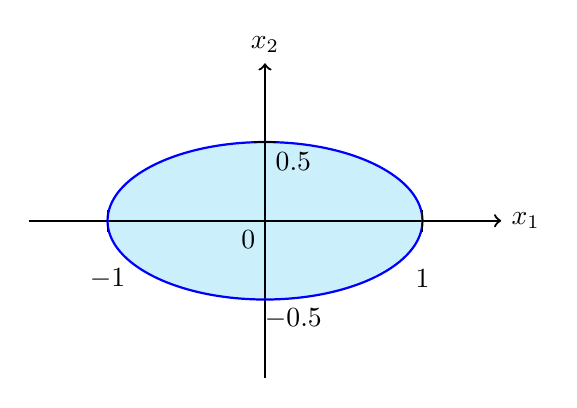
\begin{tikzpicture}[scale=2]
    % Fill the ellipse
    \fill[cyan!20] (0,0) ellipse (1cm and 0.5cm);
    
    % Draw the axes
    \draw[->, thick] (-1.5,0) -- (1.5,0) node[right] {$x_1$};
    \draw[->, thick] (0,-1) -- (0,1) node[above] {$x_2$};
    
    % Draw the ellipse boundary
    \draw[thick, color=blue] (0,0) ellipse (1cm and 0.5cm);
    
    % Add ticks and labels
    \foreach \x in {-1, 1}
        \draw (\x,0.07) -- (\x,-0.07) node[shift={(0, -0.6)}] {$\x$};
    \foreach \y in {-0.5, 0.5}
        \draw (0.07,\y) -- (-0.07,\y) node[shift={(0.5, -0.25)}] {$\y$};
    \node[below left] at (0,0) {$0$};
\end{tikzpicture}
%\caption{The unit ball $\|x\|_w \le 1$ for the weight vector $w=(1,4)$ is an ellipse centered at the origin with semi-major axis of length 1 along the $x_1$-axis and semi-minor axis of length 1/2 along the $x_2$-axis.}
\end{figure}

\subsubsection*{\normalfont}{$\therefore$ The unit ball is an ellipse defined by $x_1^2 + 4x_2^2 \le 1$, with a semi-major axis of length 1 and a semi-minor axis of length 1/2.}

\noindent\rule{\textwidth}{0.4pt}\\

\newpage

%------------------
% Solution for 5
%------------------
\subsection*{Solution 5}
\noindent\rule{\textwidth}{0.4pt}\\
\subsubsection*{Distance Table Discription}
\parbox{\textwidth}{
We are given a set of points $\mathcal{X}=\{A, B, C, D\}$ and a function $d: \mathcal{X} \times \mathcal{X} \to \mathbb{R}$ defined by the following distance table. We will determine if $d$ is a metric by checking the required axioms.
}
\begin{center}
\renewcommand{\arraystretch}{1.2}
\begin{tabular}{c|cccc}
$d(x,y)$ & A & B & C & D \\
\hline
A & 0 & 2 & 1 & 5 \\
B & 2 & 0 & 3 & 4 \\
C & 1 & 3 & 0 & 2 \\
D & 5 & 4 & 2 & 0
\end{tabular}
\end{center}

\subsubsection*{Axiom 1: Non-negativity and Identity of Indiscernibles}
\parbox{\textwidth}{
This axiom requires that $d(x, y) \geq 0$ for all $x, y \in \mathcal{X}$, and that $d(x, y) = 0$ if and only if $x = y$.
\begin{itemize}
    \item \textbf{Non-negativity:} All entries in the table are non-negative, so this condition holds.
    \item \textbf{Identity:} The diagonal entries are all zero, so $d(x, x) = 0$. All off-diagonal entries are strictly positive, so $d(x, y) > 0$ when $x \neq y$.
\end{itemize}
Hence, $d$ satisifies the first axiom (non-negativity \& identity of indiscernibles).
}

\subsubsection*{Axiom 2: Symmetry}
\parbox{\textwidth}{
This axiom requires that $d(x, y) = d(y, x)$ for all $x, y \in \mathcal{X}$. Using the distance table above we can look up the folowiing:
\begin{itemize}
    \item $d(A, B) = 2 = d(B, A)$
    \item $d(A, C) = 1 = d(C, A)$
    \item $d(A, D) = 5 = d(D, A)$
    \item $d(B, C) = 3 = d(C, B)$
    \item $d(B, D) = 4 = d(D, B)$
    \item $d(C, D) = 2 = d(D, C)$
\end{itemize}
Hence, $d$ satisifies the second axiom (symmetry).
}

\subsubsection*{Axiom 3: The Triangle Inequality}
\parbox{\textwidth}{
This axiom requires that for any three points $x, y, z \in \mathcal{X}$, the inequality $d(x, z) \leq d(x, y) + d(y, z)$ must hold. \\
Let $x=A$, $y=C$, and $z=D$.
}
\begin{align*}
    d(x, z) &\leq d(x, y) + d(y, z) \\
    d(A, D) &\leq d(A, C) + d(C, D) \\
    5 &\leq 1 + 2 \\
    5 &\leq 3 \quad (\textbf{False})
\end{align*}
\parbox{\textwidth}{
Hence, the triangle inequality does not hold, and $d$ fails the third axiom.
}

\subsubsection*{\normalfont}{$\therefore$ The function $d$ is not a metric because it fails the triangle inequality.}

\noindent\rule{\textwidth}{0.4pt}\\

\newpage

%------------------
% Solution for 6(a)
%------------------
%%%
\subsection*{Solution 6}
\noindent\rule{\textwidth}{0.4pt}\\
\subsubsection*{Solution 6 (a)}

\subsubsection*{Find Largest Possible Value of $K(p, q)$}

\parbox{\textwidth}{
Given $|\mathcal{X}| = 2$. This means that $\mathcal{X}$ is a set containing two elements. \\

Let $\mathcal{X} = \{0,1\}$, $p=(1, 0)$ and $q=(0, 1)$. \\
$p=(1, 0)$: $p(x_1)=1$, $p(x_2)=0$ \\
$q=(0, 1)$: $q(x_1)=0$, $q(x_2)=1$ \\
\begin{align*}
    K(p, q) &= p(x_1) \log\frac{p(x_1)}{q(x_1)} + p(x_2) \log\frac{p(x_2)}{q(x_2)} \\
    &= 1 \cdot \log\frac{1}{0} + 0 \cdot \log\frac{0}{1} \\
    &= \infty + 0 \\
    &= \infty
\end{align*}
}
\subsubsection*{\normalfont}{$\therefore$ The largest possible value of the KL divergence is $\infty$.}


\noindent\rule{\textwidth}{0.4pt}\\

\newpage

%------------------
% Solution for 6(b)
%------------------
%%%
\subsection*{Solution 6}
\noindent\rule{\textwidth}{0.4pt}\\
\subsubsection*{Solution 6 (b)}


\subsubsection*{Show $K(p, q)$ Non-Symmetry}
\begin{flushleft}
  Let $p = (1/2, 1/2)$ and $q = (1, 0)$
\end{flushleft}
\begin{enumerate}
  \item Compute $K(p,q)$
  \begin{align*}
    K(p, q) &= p(x_1) \log\frac{p(x_1)}{q(x_1)} + p(x_2) \log\frac{p(x_2)}{q(x_2)} \\
    &= \frac{1}{2} \log\frac{1/2}{1} + \frac{1}{2} \log\frac{1/2}{0} \\
    &= \frac{1}{2} \log\frac{1}{2} + \infty \\
    &= \infty
\end{align*}
  \item Compute $K(q,p)$
  \begin{align*}
    K(q, p) &= q(x_1) \log\frac{q(x_1)}{p(x_1)} + q(x_2) \log\frac{q(x_2)}{p(x_2)} \\
    &= 1 \cdot \log\frac{1}{1/2} + 0 \cdot \log\frac{0}{1/2} \\
    &= \log(2) + 0 \\
    &= \log(2)
\end{align*}
\begin{flushleft}
  Hence, $\infty \neq \log(2)$
\end{flushleft}
\end{enumerate}

\subsubsection*{\normalfont}{$\therefore$ $K(p, q) \neq K(q, p)$, and the KL divergence is not symmetric.}

\noindent\rule{\textwidth}{0.4pt}\\

\newpage

%------------------
% Solution for 7
%------------------
\subsection*{Solution 7}
\noindent\rule{\textwidth}{0.4pt}\\

\subsubsection*{Define Jaccard Similarity}
\parbox{\textwidth}{
Jaccard similarity between two sets $A$ and $B$ is the following:

$$J(A,B) = \frac{|A \cap B|}{|A \cup B|}$$
}
\subsubsection*{Compute Jaccard Similarity}
\parbox{\textwidth}{
Let $A = \{1, 3, 5, 7, 9\}$ and $B = \{2, 3, 5, 7\}$

\begin{align*}
    J(A, B) &= \frac{|A \cap B|}{|A \cup B|} \\
    &= \frac{|\{1, 3, 5, 7, 9\} \cap \{2, 3, 5, 7\}|}{|\{1, 3, 5, 7, 9\} \cup \{2, 3, 5, 7\}|} \\
    &= \frac{|\{3, 5, 7\}|}{|\{1, 2, 3, 5, 7, 9\}|} \\
    &= \frac{3}{6} \\
    &= \frac{1}{2}
\end{align*}
}

\subsubsection*{\normalfont}{$\therefore$ The Jaccard similarity $J(A, B)$ is $\frac{1}{2}$ or 50\%.}

\noindent\rule{\textwidth}{0.4pt}\\

\newpage

%------------------
% Solution for 8
%------------------
%%%
\subsection*{Solution 8}
\noindent\rule{\textwidth}{0.4pt}\\
\subsubsection*{Convert Sentences to Bigrams}
\parbox{\textwidth}{
Let: \\
\\
$x$: ''Napoleon was born in 1769'' $\rightarrow$ $B(x) = \{(\text{Napoleon, was}), (\text{was, born}), (\text{born, in}), (\text{in, 1769})\}$
\\
$x^{\prime}$: ''Napoleon was born when'' $\rightarrow$ $B(x^{\prime}) = \{(\text{Napoleon, was}), (\text{was, born}), (\text{born, when})\}$
\\
The Jaccard similarity for the bigram sets $B(x)$ and $B(x^{\prime})$ is defined as:
$$J(B(x), B(x^{\prime})) = \frac{|B(x) \cap B(x^{\prime})|}{|B(x) \cup B(x^{\prime})|}$$
}

\subsubsection*{Compute Jaccard Similarity}
\begin{align*}
    &J(B(x), B(x^{\prime})) = \frac{|B(x) \cap B(x^{\prime})|}{|B(x) \cup B(x^{\prime})|} \\
    &= \frac{|\{(\text{Napoleon, was}), (\text{was, born}), (\text{born, in}), (\text{in, 1769})\} \cap \{(\text{Napoleon, was}), (\text{was, born}), (\text{born, when})\}|}{|\{(\text{Napoleon, was}), (\text{was, born}), (\text{born, in}), (\text{in, 1769})\}\cup \{(\text{Napoleon, was}), (\text{was, born}), (\text{born, when})\}|} \\
    &= \frac{|\{(\text{Napoleon, was}), (\text{was, born})\}|}{|\{(\text{Napoleon, was}), (\text{was, born}), (\text{born, when}),(\text{born, in}), (\text{in, 1769})\}|} \\
    &= \frac{2}{5} 
\end{align*}


\subsubsection*{\normalfont}{$\therefore$ The Jaccard similarity $J(B(x), B(x^{\prime}))$ is $\frac{2}{5}$ or 40\%.}

\noindent\rule{\textwidth}{0.4pt}\\

\newpage

%------------------
% Solution for 9 (a)
%------------------
\subsection*{Solution 9}
\noindent\rule{\textwidth}{0.4pt}\\
\subsubsection*{Solution 9 (a)}
\subsubsection*{Define Cosine Similarity}
\parbox{\textwidth}{
  The cosine similarity between two vectors $x$ and $y$ is defined as:
  $$\text{cos}(\theta) = \frac{x \cdot y}{||x|| ||y||} = \frac{\sum_{i=1}^{n}x_{i}y_{i}}{\sqrt{\sum_{i=1}^{n}x_{i}^2}\sqrt{\sum_{i=1}^{n}y_{i}^2}}$$
}
\subsubsection*{Compute Cosine Similarity}
\parbox{\textwidth}{
  Let $x=\begin{bmatrix} 1 \\ 2 \\ 3 \end{bmatrix}$ and $x^{\prime}=\begin{bmatrix} 1 \\ 2 \\ 3 \end{bmatrix}$

}
\begin{align*}
    \text{cos}(\theta) &= \frac{x \cdot x^{\prime}}{||x|| ||x^{\prime}||} \\
    &= \frac{\sum_{i=1}^{n}x_{i}x^{\prime}_{i}}{\sqrt{\sum_{i=1}^{n}x_{i}^2}\sqrt{\sum_{i=1}^{n}{x^{\prime}}_{i}^2}} \\
    &= \frac{(1)(3) + (2)(2) + (3)(1)}{\sqrt{1^2+2^2+3^2} \sqrt{3^2+2^2+1^2}} \\
    &= \frac{3 + 4 + 3}{\sqrt{1+4+9} \sqrt{9+4+1}} \\
    &= \frac{10}{\sqrt{14} \sqrt{14}} \\
    &= \frac{10}{14} \\
    &= \frac{5}{7}
\end{align*}
\subsubsection*{\normalfont}{$\therefore$ The cosine similarity between $x$ and $x'$ is $\frac{5}{7}$.}


\noindent\rule{\textwidth}{0.4pt}\\

\newpage

%------------------
% Solution for 9 (b)
%------------------
\subsection*{Solution 9}
\noindent\rule{\textwidth}{0.4pt}\\
\subsubsection*{Solution 9 (b)}
\subsubsection*{(b): Characterization of Zero Similarity}
\parbox{\textwidth}{
The cosine similarity between two non-zero vectors $x$ and $x^{\prime}$ is zero if and only if the numerator of the formula is zero.
$$ \text{cos}(\theta) = 0 \iff x \cdot x^{\prime} = 0 $$
In a Euclidean vector space, a dot product of zero signifies that the two vectors are orthogonal (perpendicular) to each other. The angle $\theta$ between them is $90^\circ$ or $\frac{\pi}{2}$ radians. Geometrically, they form a right angle.
}
\subsubsection*{\normalfont}{$\therefore$ A cosine similarity of zero means the vectors are orthogonal to each other.}

\noindent\rule{\textwidth}{0.4pt}\\

\newpage
%------------------
% Solution for 9 (c)
%------------------
%%% come back.. image i dont get
\subsection*{Solution 9}
\noindent\rule{\textwidth}{0.4pt}\\
\subsubsection*{Solution 9 (c)}

\subsubsection*{Sketch of the Region}
The shaded region below represents the cone containing all vectors $y$ satisfying $cos(\theta) \geq 0.9$.
\begin{center}
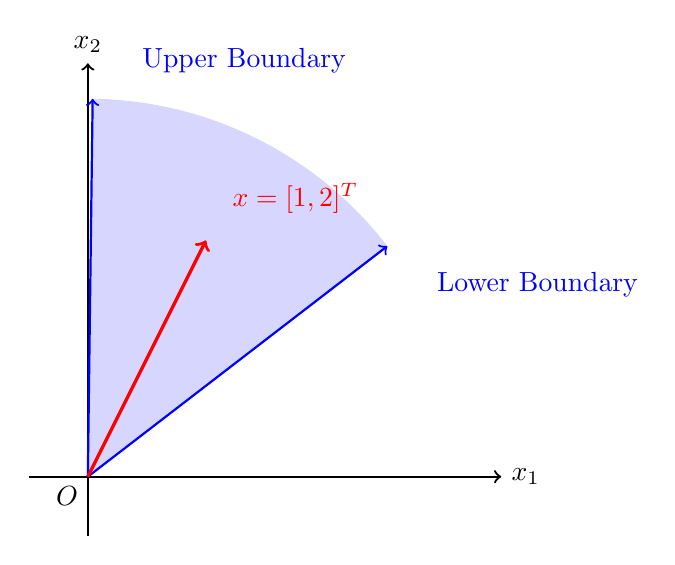
\begin{tikzpicture}[scale=1.5]
    % Define angles
    \def\phi{63.43}
    \def\thetaMax{25.84}
    \def\angleA{\phi - \thetaMax} % Lower bound angle
    \def\angleB{\phi + \thetaMax} % Upper bound angle

    % Draw axes
    \draw[->, thick] (-0.5, 0) -- (3.5, 0) node[right] {$x_1$};
    \draw[->, thick] (0, -0.5) -- (0, 3.5) node[above] {$x_2$};
    \node[below left] at (0,0) {$O$};

    % Shade the conical region
    \fill[blue!20, opacity=0.8] (0,0) -- (\angleA:3.2) arc (\angleA:\angleB:3.2) -- cycle;

    % Draw boundary vectors
    \draw[->, thick, blue] (0,0) -- (\angleA:3.2) node[below right, xshift=5mm, yshift=-2mm] {Lower Boundary};
    \draw[->, thick, blue] (0,0) -- (\angleB:3.2) node[above right, xshift=5mm, yshift=2mm] {Upper Boundary};

    % Draw the reference vector x
    \draw[->, very thick, red] (0,0) -- (1,2) node[above right, xshift=2mm, yshift=2mm] {$x=[1,2]^T$};

    % Define coordinates for angles
    \coordinate (O) at (0,0);
    \coordinate (X) at (1,0);
    \coordinate (X_vec) at (1,2);
    \coordinate (B1) at (\angleA:3.2);
    \coordinate (B2) at (\angleB:3.2);
    % idk wft anything about geometry 
    % Draw and label angles 
    % Angle phi from x_1 axis to vector x
    %\draw pic[draw, angle radius=1.2cm, pic text=$\phi$, pic text options={above=2mm, left=5mm}] {angle=X--O--X_vec};
    % Angle theta_max from vector x to lower boundary
    %\draw pic[draw, angle radius=0.7cm, pic text=$\theta_{\text{max}}$, pic text options={right=2mm}] {angle=B1--O--X_vec};
    % Angle theta_max from vector x to upper boundary
    %\draw pic[draw, angle radius=0.7cm, pic text=$\theta_{\text{max}}$, pic text options={above=2mm, right=2mm}] {angle=X_vec--O--B2};
\end{tikzpicture}
\end{center}

\noindent\rule{\textwidth}{0.4pt}\\

\newpage
%------------------
% Solution for 10 (a)
%------------------
%%%
\subsection*{Solution 10}
\noindent\rule{\textwidth}{0.4pt}\\
\subsubsection*{Solution  10 (a)}

\subsubsection*{Compute Mean}
\parbox{\textwidth}{The mean (Expected Value) $E[X]$ is calculated as the sum of each outcome weighted by its probability: 
$$E[X] = \sum_{i} x_i P(X=x_i)$$ }
\begin{align*}
E[X] &= (1)\left(\frac{1}{3}\right) + (2)\left(\frac{1}{3}\right) + (3)\left(\frac{1}{12}\right) + (4)\left(\frac{1}{12}\right) + (5)\left(\frac{1}{12}\right) + (6)\left(\frac{1}{12}\right) \\
&= \frac{4}{12} + \frac{8}{12} + \frac{3}{12} + \frac{4}{12} + \frac{5}{12} + \frac{6}{12} \\
&= \frac{30}{12} = \frac{5}{2} = 2.5
\end{align*}
\subsubsection*{Compute Median}
\parbox{\textwidth}{The median is the value $x_m$ for which the cumulative probability $P(X \le x_m)$ first equals or exceeds 0.5.
\begin{align*}
P(X \le 1) &= \frac{1}{3} \\
P(X \le 2) &= \frac{1}{3} + \frac{1}{3} = \frac{2}{3} 
\end{align*}
Hence, $P(X \le 2)$ is the first cumulative probability to exceed 0.5, and the median is 2.}
\subsubsection*{\normalfont}{$\therefore$ The mean is $2.5$ and the median is $2$.}

\noindent\rule{\textwidth}{0.4pt}\\

\newpage
%------------------
% Solution for 10 (b)
%------------------
%%%
\subsection*{Solution 10}
\noindent\rule{\textwidth}{0.4pt}\\
\subsubsection*{Compute Variance}

\parbox{\textwidth}{Variance is defined as:
$$\text{Var}(X) = E[X^2] - (E[X])^2\text{, where } E[X^2] = \sum_{i} x_i^2 P(X=x_i)$$ 
}
\begin{align*}
E[X^2] &= (1^2)\left(\frac{1}{3}\right) + (2^2)\left(\frac{1}{3}\right) + (3^2)\left(\frac{1}{12}\right) + (4^2)\left(\frac{1}{12}\right) + (5^2)\left(\frac{1}{12}\right) + (6^2)\left(\frac{1}{12}\right) \\
&= \frac{4}{12} + \frac{16}{12} + \frac{9}{12} + \frac{16}{12} + \frac{25}{12} + \frac{36}{12} \\
&= \frac{106}{12} = \frac{53}{6} \\
\\
\text{Var}(X) &= E[X^2] - (E[X])^2 = \frac{53}{6} - \left(\frac{5}{2}\right)^2 \\
&= \frac{53}{6} - \frac{25}{4} = \frac{106}{12} - \frac{75}{12} = \frac{31}{12} 
\end{align*}
\subsubsection*{Compute Standard Deviation}

\parbox{\textwidth}{The standard deviation is the square root of the variance:
$$\text{SD}(X) = \sqrt{\text{Var}(X)}$$

It follows that, $\text{SD}(X) = \sqrt{\frac{31}{12}}$
}
\subsubsection*{\normalfont}{$\therefore$ The theoretical variance is $\text{Var}(X) = \frac{31}{12}$ and the standard deviation is $\text{SD}(X) = \sqrt{\frac{31}{12}}$.}


\noindent\rule{\textwidth}{0.4pt}\\

\newpage

%------------------
% Solution for 10 (c)
%------------------
%%%
\subsection*{Solution 10}
\noindent\rule{\textwidth}{0.4pt}\\
\subsubsection*{Solution  10 (c)}
\parbox{\textwidth}{Given the set of $N=10$ observations $D = \{2, 5, 1, 4, 2, 2, 5, 6, 1, 2\}$, the empirical probability is defined as:
 $$\hat{P}(X=x) = \frac{|x|}{N} \text{where }|x| \text{ is frequency of event x in set D}$$ 
}
\parbox{\textwidth}{The counts for each outcome are: \\ Count(1) = 2 \\ Count(2) = 4 \\ Count(3) = 0 \\ Count(4) = 1 \\ Count(5) = 2 \\ Count(6) = 1 \\

Hence the probabilities for each event are:
$$ \hat{P}(1)=0.2 \text{, } \hat{P}(2)=0.4 \text{, } \hat{P}(3)=0.0 \text{, } \hat{P}(4)=0.1 \text{, }  \hat{P}(5)=0.2 \text{, } \hat{P}(6)=0.1$$
}

\subsubsection*{\normalfont $\therefore$ The empirical distribution is the following:}

% Use the standard LaTeX display math environment \[ ... \]
\[
P(X=x) =
\begin{cases}
    0.2 & \text{if } x=1 \\
    0.4 & \text{if } x=2 \\
    0.0 & \text{if } x=3 \\
    0.1 & \text{if } x=4 \\
    0.2 & \text{if } x=5 \\
    0.1 & \text{if } x=6
\end{cases}
\]


\noindent\rule{\textwidth}{0.4pt}\\

\newpage

%------------------
% Solution for 10 (d)
%------------------
%%%
\subsection*{Solution 10}
\noindent\rule{\textwidth}{0.4pt}\\
\subsubsection*{Solution  10 (d)}
\parbox{\textwidth}{The empirical mean is $\bar{x} = \frac{1}{N}\sum x_i$. The median is the middle value of the sorted data. The empirical variance is $\text{Var} = \frac{1}{N}\sum(x_i - \bar{x})^2$, and the standard deviation is $\text{SD} = \sqrt{\text{Var}}$.}
\subsubsection*{Compute Mean}
$$\bar{x} = \frac{1}{10}(2+5+1+4+2+2+5+6+1+2) = \frac{30}{10} = 3.0$$

\subsubsection*{Compute Median}
\parbox{\textwidth}{Sorted data: $\{1, 1, 2, 2, \textbf{2, 2}, 4, 5, 5, 6\}$. The median is the average of the 5th and 6th values: $\frac{2+2}{2} = 2$.}
\subsubsection*{Compute Variance and Standard Deviation}

\begin{align*}
\text{Var} &= \frac{1}{10}\sum_{i=1}^{10}(x_i - 3.0)^2 \\
&= \frac{1}{10}\left[(1-3)^2 \times 2 + (2-3)^2 \times 4 + (4-3)^2 \times 1 + (5-3)^2 \times 2 + (6-3)^2 \times 1\right] \\
&= \frac{1}{10}\left[(-2)^2 \times 2 + (-1)^2 \times 4 + (1)^2 \times 1 + (2)^2 \times 2 + (3)^2 \times 1\right] \\
&= \frac{1}{10}\left[4 \times 2 + 1 \times 4 + 1 \times 1 + 4 \times 2 + 9 \times 1\right] \\
&= \frac{1}{10}\left[8 + 4 + 1 + 8 + 9\right] = \frac{30}{10} \\
&= 3 
\\
SD &= \sqrt{3} 
\end{align*}
\subsubsection*{\normalfont}{$\therefore$ The empirical mean is $\bar{x}=3.0$, median is $2$, variance is $\text{Var}=3$, and standard deviation is $SD = \sqrt{3}$.}


\noindent\rule{\textwidth}{0.4pt}\\

\newpage

%------------------
% Solution for 11 (a)
%------------------
\subsection*{Solution 11}
\noindent\rule{\textwidth}{0.4pt}\\
\subsubsection*{Solution  11 (a)}

\parbox{\textwidth}{
    \textbf{Justification:} The distribution of human height for a given population (e.g., adult males) is famously well-approximated by a symmetric, bell-shaped curve (a Normal or Gaussian distribution). In a perfectly symmetric distribution, the mean, median, and mode coincide. Therefore, the center of mass (mean) and the geometric center (median) are expected to be nearly identical.
}

\subsubsection*{\normalfont $\therefore$ We expect $\text{Mean}(H) \approx \text{Median}(H)$. No significant difference.}

\noindent\rule{\textwidth}{0.4pt}\\

\newpage
%------------------
% Solution for 11 (b)
%------------------
\subsection*{Solution 11}
\noindent\rule{\textwidth}{0.4pt}\\
\subsubsection*{Solution  11 (b)}

\parbox{\textwidth}{
    \textbf{Justification:} The distribution of housing costs is almost always characterized by a strong right-skew. Most houses fall within a certain price range, there is a long tail of extremely expensive properties. These high-value outliers pull the mean significantly upward, while the median remains a more robust measure of the "typical" house price, unaffected by these extreme values.
}

\subsubsection*{\normalfont $\therefore$ We expect $\text{Mean}(C) > \text{Median}(C)$. A significant difference.}

\noindent\rule{\textwidth}{0.4pt}\\

\newpage

%------------------
% Solution for 11 (c)
%------------------
\subsection*{Solution 11}
\noindent\rule{\textwidth}{0.4pt}\\
\subsubsection*{Solution  11 (c)}

\parbox{\textwidth}{
    \textbf{Justification:} The distribution of GPAs is often left-skewed. This is due to a "ceiling effect," where a large number of students achieve high grades clustered near the maximum possible GPA ($\approx$ 4.0), while fewer students have very low GPAs. This clustering at the high end pulls the median towards the right, while the lower-end scores pull the mean to the left.
}

\subsubsection*{\normalfont $\therefore$ We expect $\text{Mean}(G) < \text{Median}(G)$, but the difference may not be as significant as for  house cost or salary.}

\noindent\rule{\textwidth}{0.4pt}\\

\newpage
%------------------
% Solution for 11 (d)
%------------------
\subsection*{Solution 11}
\noindent\rule{\textwidth}{0.4pt}\\
\subsubsection*{Solution  11 (d)}

\parbox{\textwidth}{
    \textbf{Justification:} Similar to housing costs, salary data exhibits a pronounced right-skew. The majority of people earn modest. However, a small number of individuals (CEOs, top athletes, etc.) have high incomes. These outliers have strong influence on the mean, that pulls it far to the right of the median. The median salary is therefore a much more accurate representation of a typical worker's salary.
}
\vspace{1em}
\subsubsection*{\normalfont $\therefore$ We expect $\text{Mean}(S) > \text{Median}(S)$. A significant difference.}


\noindent\rule{\textwidth}{0.4pt}\\

\newpage
%------------------
% Solution for 12
%------------------
\subsection*{Solution 12}
\noindent\rule{\textwidth}{0.4pt}\\
\subsubsection*{Define relationships}

\parbox{\textwidth}{
We know the following relationships are true:
$$ Var[Z] = E[Z^2] - (E[Z])^2$$
$$\sigma^{2} = \text{Var}[Z]$$ 
$$E[Z] = \mu$$
Rearranging this formula allows us to solve for $E[Z^2]$:
$$ E[Z^2] = Var[Z] + (E[Z])^2 = \sigma^2 + \mu^2 $$

}
\subsubsection*{Compute $E[Z^{2}]$}
\parbox{\textwidth}{
Given: $\mu = E[Z] = -1$ and the standard deviation $SD[Z] = \sigma = 2$
}
\begin{align*}
E[Z^2] &= \sigma^2 + \mu^2 \\
&= (2)^2 + (-1)^2 \\
&= 4 + 1 \\
&= 5
\end{align*}

\subsubsection*{\normalfont}{$\therefore$ $E[Z^2]$ is 5.}

\noindent\rule{\textwidth}{0.4pt}\\

\newpage

%------------------
% Solution for 13 (a)
%------------------
\subsection*{Solution 13}
\noindent\rule{\textwidth}{0.4pt}\\
\subsubsection*{Solution  13 (a)}
\subsubsection*{Define X and Y Independence}
\parbox{\textwidth}{
Two discrete random variables $X$ and $Y$ are independent if and only if $P(X=x, Y=y) = P(X=x)P(Y=y)$ for all possible pairs $(x, y)$.
\subsubsection*{Compute Marginal Probability Mass Functions}


 We sum rows and columns of the joint PMF table to compute $P(X=x)$ and $P(Y=y)$.
\begin{align*}
    P(X=1) &= 0.10 + 0.20 + 0.05 = 0.35 \\
    P(X=2) &= 0.10 + 0.15 + 0.05 = 0.30 \\
    P(X=3) &= 0.10 + 0.15 + 0.10 = 0.35
\end{align*}
\begin{align*}
    P(Y=1) &= 0.10 + 0.10 + 0.10 = 0.30 \\
    P(Y=2) &= 0.20 + 0.15 + 0.15 = 0.50 \\
    P(Y=3) &= 0.05 + 0.05 + 0.10 = 0.20
\end{align*}
}
\vspace{1em}
\subsubsection*{Test Independence Condition}
The test below is the independence condition for the pair $(X=1, Y=1)$:
\begin{align*}
    P(X=1, Y=1) &\stackrel{?}{=} P(X=1)P(Y=1) \\
    0.10 &\stackrel{?}{=} (0.35)(0.30) \\
    0.10 &\neq 0.105
\end{align*}

\subsubsection*{\normalfont{$\therefore$ Since the joint probability $P(X=1, Y=1)$ does not equal the product of the marginal probabilities $P(X=1)P(Y=1)$, the random variables $X$ and $Y$ are NOT independent.}}

\noindent\rule{\textwidth}{0.4pt}\\

\newpage
%------------------
% Solution for 13 (b)
%------------------
\subsection*{Solution 13}
\noindent\rule{\textwidth}{0.4pt}\\
\subsubsection*{Solution  13 (b)}

\subsubsection*{Define Covariance and Correlation of X and Y}
\parbox{\textwidth}{
The covariance is as follows:
$$\text{Cov}[X, Y] = E[XY] - E[X]E[Y]$$
The correlation is as follows
$$\rho_{X, Y} = \frac{\text{Cov}[X, Y]}{\sigma_X \sigma_Y}$$
}

\subsubsection*{Compute Expectations $X$ $Y$ and $XY$}

\begin{align*}
  E[X] &= \sum_{x} x P(X=x) = 1(0.35) + 2(0.30) + 3(0.35) = 0.35 + 0.60 + 1.05 = 2.0 \\
  E[Y] &= \sum_{y} y P(Y=y) = 1(0.30) + 2(0.50) + 3(0.20) = 0.30 + 1.00 + 0.60 = 1.9 \\
    E[XY] &= \sum_{x,y} xy P(X=x, Y=y) \\
          &= (1)(1)(0.10) + (1)(2)(0.20) + (1)(3)(0.05) \\
          &\quad + (2)(1)(0.10) + (2)(2)(0.15) + (2)(3)(0.05) \\
          &\quad + (3)(1)(0.10) + (3)(2)(0.15) + (3)(3)(0.10) \\
          &= 0.10 + 0.40 + 0.15 + 0.20 + 0.60 + 0.30 + 0.30 + 0.90 + 0.90 \\
          &= 3.85
\end{align*}

\subsubsection*{Compute Covariance}
$$\text{Cov}[X, Y] = E[XY] - E[X]E[Y] = 3.85 - (2.0)(1.9) = 3.85 - 3.80 = 0.05$$

\subsubsection*{Compute Variances and Standard Deviations}
\begin{align*}
    E[X^2] &= 1^2(0.35) + 2^2(0.30) + 3^2(0.35) = 0.35 + 1.20 + 3.15 = 4.7 \\
    \text{Var}[X] &= E[X^2] - (E[X])^2 = 4.7 - 2.0^2 = 0.7 \\
    \sigma_X &= \sqrt{0.7} \\
    \\
    E[Y^2] &= 1^2(0.30) + 2^2(0.50) + 3^2(0.20) = 0.30 + 2.00 + 1.80 = 4.1 \\
    \text{Var}[Y] &= E[Y^2] - (E[Y])^2 = 4.1 - 1.9^2 = 4.1 - 3.61 = 0.49 \\
    \sigma_Y &= \sqrt{0.49}
\end{align*}

\subsubsection*{Compute Correlation Coefficient}
$$\rho_{X, Y} = \frac{\text{Cov}[X, Y]}{\sigma_X \sigma_Y} = \frac{0.05}{\sqrt{0.7} \cdot \sqrt{0.49}} \approx 0.0854$$

\subsubsection*{\normalfont{$\therefore$ The covariance is $\text{Cov}[X, Y] = 0.05$, and the correlation coefficient is $\rho_{X, Y} \approx 0.0854$. This indicates a very weak positive linear relationship between $X$ and $Y$.}}

\noindent\rule{\textwidth}{0.4pt}\\

\newpage

%------------------
% Solution for 14 (a)
%------------------
\subsection*{Solution 14}
\noindent\rule{\textwidth}{0.4pt}\\
\subsubsection*{Solution  14 (a)}
\parbox{\textwidth}{
The expectation of $Y$, $E[Y]$, via the linearity of expectation is defined as:
$$ E[Y] = E[aX + b] = aE[X] + b $$
The covariance between $X$ and $Y$ is defined as:
$$\text{Cov}[X, Y] = E[(X - E[X])(Y - E[Y])]$$
Now,substitute the expression for $E[Y]$ into the expression for covariance:
}
\begin{align*}
\text{Cov}[X, Y] &= E\left[ (X - E[X])(Y - E[Y]) \right] \\
&= E\left[ (X - E[X])((aX + b) - (aE[X] + b)) \right] \\
&= E\left[ (X - E[X])(aX + b - aE[X] - b) \right] \\
&= E\left[ (X - E[X])(aX - aE[X]) \right] \\
&= E\left[ (X - E[X])a(X - E[X]) \right] \\
&= a \cdot E\left[ (X - E[X])^2 \right] \\
&= a \cdot \text{Var}[X]
\end{align*}

\subsubsection*{\normalfont}{$\therefore$ The covariance between $X$ and $Y$ ,in terms of $X$ is the following:}
$$\text{Cov}[X, Y] = a \cdot \text{Var}[X]$$


\noindent\rule{\textwidth}{0.4pt}\\

\newpage
%------------------
% Solution for 14 (b)
%------------------
\subsection*{Solution 14}
\noindent\rule{\textwidth}{0.4pt}\\
\subsubsection*{Solution  14 (b)}

\subsubsection*{Part (b): Deriving the Correlation $\rho_{X, Y}$}
\parbox{\textwidth}{
The correlation coefficient $\rho_{X, Y}$ is defined as:
$$\rho_{X, Y} = \frac{\text{Cov}[X, Y]}{\text{SD}[X]\text{SD}[Y]}$$
The variance of $Y$ is the following:
$$ \text{Var}[Y] = \text{Var}[aX + b] = a^2 \text{Var}[X] $$
First, we need find the standard deviation of $Y$:
$$ \text{SD}[Y] = \sqrt{\text{Var}[Y]} = \sqrt{a^2 \text{Var}[X]} = |a|\sqrt{\text{Var}[X]} = |a| \cdot \text{SD}[X] $$
Now, substitute the known quantities into the correlation formula:
}
\begin{align*}
\rho_{X, Y} &= \frac{\text{Cov}[X, Y]}{\text{SD}[X]\text{SD}[Y]} \\
&= \frac{a \cdot \text{Var}[X]}{\text{SD}[X] \cdot (|a| \cdot \text{SD}[X])} \\
&= \frac{a \cdot (\text{SD}[X])^2}{|a| \cdot (\text{SD}[X])^2} \\
&= \frac{a}{|a|} 
\end{align*}

\subsubsection*{\normalfont}{$\therefore$ The correlation between $X$ and $Y$ is $\rho_{X, Y} = \frac{a}{|a|}$, which is $1$ if $a>0$, $-1$ if $a<0$, and undefined if $a=0$.}


\noindent\rule{\textwidth}{0.4pt}\\

\newpage

\subsection*{Solution 15}
\noindent\rule{\textwidth}{0.4pt}\\
\vspace{1em}

\begin{flushleft}
    Two random variables $X$ and $Y$ are uncorrelated if their covariance is zero. The covariance is defined as:
    $$ \text{Cov}[X, Y] = E[XY] - E[X]E[Y] $$
    We first calculate the expected value of $X$, $E[X]$.
\end{flushleft}
\begin{align*}
    E[X] &= \sum_{x \in \Omega_X} x \cdot P(X=x) \\
         &= (-1) \cdot P(X=-1) + (0) \cdot P(X=0) + (1) \cdot P(X=1) \\
         &= (-1) \cdot \frac{1}{3} + (0) \cdot \frac{1}{3} + (1) \cdot \frac{1}{3} \\
         &= -\frac{1}{3} + 0 + \frac{1}{3} \\
         &= 0
\end{align*}
\parbox{\textwidth}{
    Since $E[X] = 0$, the covariance formula simplifies significantly:
    $$ \text{Cov}[X, Y] = E[XY] - (0) \cdot E[Y] = E[XY] $$
    Hence, for $X$ and $Y$ to be uncorrelated, we only need to find a function $f$ such that:
    $$E[X f(X)] = 0$$\\
    Next we expand the  condition $E[X f(X)] = 0$:\\
    $$ E[X f(X)] = \sum_{x \in \Omega_X} x f(x) P(X=x) = \frac{1}{3} \left( (-1)f(-1) + (0)f(0) + (1)f(1) \right) = 0 $$
    This implies that we need $-f(-1) + f(1) = 0$, or $f(-1) = f(1)$.\\

    Let $f(x) = x^{2}$ and verify that $E[XY] = 0$.
}

\begin{align*}
    E[XY] &= E[X \cdot X^2] = E[X^3] \\
          &= \sum_{x \in \Omega_X} x^3 \cdot P(X=x) \\
          &= (-1)^3 \cdot P(X=-1) + (0)^3 \cdot P(X=0) + (1)^3 \cdot P(X=1) \\
          &= (-1) \cdot \frac{1}{3} + (0) \cdot \frac{1}{3} + (1) \cdot \frac{1}{3} \\
          &= -\frac{1}{3} + 0 + \frac{1}{3} \\
          &= 0
\end{align*}

\begin{flushleft}
    For $Y = f(X) = X^{2}$ we have $E[XY] = 0$ and $E[X]=0$, and $\text{Cov}[X, Y] = 0$. The variable $Y=X^2$ is determined by $X$, yet they are linearly uncorrelated.
\end{flushleft}

\subsubsection*{\normalfont{$\therefore$ the function is $f(X) = X^{2}$}}

\noindent\rule{\textwidth}{0.4pt}\\

\end{document}